\documentclass[10pt,letterpaper]{article}
\usepackage{tools}
\usepackage{xepersian}
\usepackage{enumitem}
%\settextfont{B Nazanin}
\usepackage{lipsum}
\setlength{\parskip}{3mm}
\setlength{\parindent}{0mm}
\begin{document}
\Large
\begin{center}
امتحان پایانترم درس شبکه های مخابراتی

مدت زمان: 100 دقیقه

\hrulefill
\end{center}
سوال 1) یک کاربر برای مشاهده‌ی صفحه‌ی وب خاصی که شامل 10 تصویر هر یک با حجم 
$
12.5Kbytes
$
است، درخواست می دهد. مطابق شکل زیر بین کاربر و سرور، دو لینک و یک روتر وجود دارد. اگر طول هر لینک 50 کیلومتر، نرخ ارسال روی لینک های 1 و 2 به ترتیب 
$
1000 Kbps
$
 و
$
500 Kbps
$
و درخواست از نوع 
persistent
باشد، چقدر طول می کشد که کاربر بتواند صفحه‌ی وب را با تمام تصاویر داخل آن دانلود کند؟

(حجم درخواست ها و صفحه‌ی HTTP را ناچیز در نظر بگیرید. همچنین تاخیر صف و پردازش روتر برابر صفر و سرعت نور 
$
2\times 10^8 \text{m/s}
$
است.)
\begin{figure}[htb]
\centering
\includegraphics[width=160mm]{http.pdf}
\end{figure}
\newpage
سوال 2) فرض کنید فرستنده ای، 4 بسته با شماره‌های 0، 1، 2 و 3 را به ترتیب و پشت سر هم ارسال می کند. بسته‌ی شماره‌ی 2 به گیرنده نمیرسد و بسته‌ی شماره‌ی 1 نیز به مقصد رسیده، ولی ACK آن در کانال از بین می رود. توضیح دهید هر یک از الگوریتم های 
GBN
و
SR
چه عملکردی را از خود نشان می دهند.
\begin{figure}[htb]
\centering
\includegraphics[width=160mm]{gbn_sr.pdf}
\end{figure}
\newpage
سوال 3) 

الف) در شبکه‌ی زیر، بین نودهای A (مبدا) و Z (مقصد) کوتاهترین مسیر را به کمک الگوریتم دایکسترا (\lr{Dijkstra's Algorithm}) بیابید (فرایند این الگوریتم را به صورت کامل و در قالب جدول بنویسید).

ب) فرض کنید برای تعیین کوتاهترین مسیر بین نودهای A و Z در شبکه‌ی زیر، از الگوریتم 
\lr{Distance Vector}
استفاده کرده ایم. اکنون هزینه‌ی لینک BZ ، از 1 به 5 افزایش می یابد. توضیح دهید جهت پیدا کردن مسیر بهینه‌ی جدید بین A و Z، الگوریتم 
\lr{Distance Vector}
به چه مشکلی بر می خورد؟ راه حل این مشکل چیست؟
\begin{figure}[htb]
\centering
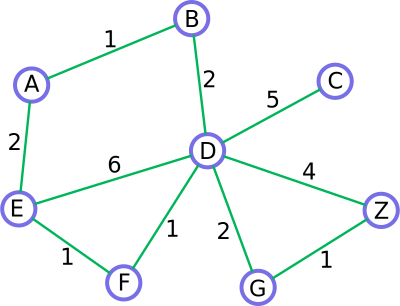
\includegraphics[width=160mm]{dij.pdf}
\end{figure}
\newpage
سوال 4) در شبکه ای با توپولوژی زیر، فرض کنید نود A می خواهد بسته ای به حجم 
\lr{5 Kbytes}
را به سایر نودها پخش 
(\lr{Broadcast})
کند. چه مقدار حجم داده در تمام لینک های شبکه استفاده خواهد شد اگر برای 
\lr{Broadcast}
کردن:

الف) از
\lr{Uncontrolled Flooding}
استفاده شود؟

ب) از
\lr{Controlled Flooding}
با روش 
\lr{reverse path forwarding}
استفاده شود؟

پ) از 
\lr{Minimum Spanning Tree}
 با روش 
\lr{center-based}
استفاده شود؟ (همچنین مراحل ساخت درخت را توضیح دهید.)

(هزینه تمام لینک ها برابر 1 است)
\begin{figure}[htb]
\centering
\includegraphics[width=130mm]{broadcast.pdf}
\end{figure}
\newpage
سوال 5) در دیاگرام فضا-زمان زیر برای پروتکل
\lr{CSMA/CD}
، دو نود B و D پس از آشکار سازی تصادم بسته‌ها 
(\lr{Collision Detection})
، از روش 
\lr{binary exponential backoff}
برای تعیین زمان تصادفی ارسال خود استفاده می کنند. نودها پس از اندازه گیری 
$
n
$
تصادم بسته‌ی خود، زمان تصادفی ای در بازه‌ی 
$
\{0,1,2,\cdots,2^{n}-1\}\times 1msec
$
مستقل از هم انتخاب کرده و پس از سپری شدن زمان انتخاب شده‌ی خود، اقدام به ارسال مجدد بسته ها می کنند. اگر هر نود برای ارسال هر بسته‌ی خود به 1 میلی ثانیه زمان نیاز داشته باشد،

الف) 
%با چه احتمالی نود $B$، 2 بار 
%\lr{collision}
%را برای بسته‌ی خود تجربه می کند و در بار سوم موفق به ارسال بسته می شود؟
با چه احتمالی نود $B$ پس از 1 بار تجربه کردن
\lr{collision}
،  در بار دوم موفق به ارسال بسته می‌شود؟

ب) احتمال اینکه هر دو نود در 5 ارسال اول دچار 
\lr{collision}
شوند، چقدر است؟

(فرض کنید هر دو نود در زمان صفر اقدام به ارسال بسته‌ی خود می کنند و تصادم اول رخ می‌دهد. هر نود پس از ارسال موفق هر بسته، بلافاصله ارسال بسته‌ی بعدی را شروع می کند. همچنین سایر تاخیرها از جمله تاخیر 
\lr{collision detection}
را صفر در نظر بگیرید.)
\begin{figure}[htb]
\centering
\includegraphics[width=130mm]{csma_cd.png}
\end{figure}
\end{document}